\section{Bias-Variance Tradeoff and dealing with model complexity}
\thispagestyle{plain}

We are again starting with some sample data $\mathcal{D} = \{(\vec{x}_i, y_i)\}_{i=1}^n$
which we assume to have been generated by a model
\begin{equation}
    y = f_{\vec{\theta}^\star}(\vec{x}) + \epsilon
\end{equation}

\bluebox{\textbf{Aim:} For unseen data, we want to predict $y$ from $\vec{x}$ as accurately as possible.}

\greenbox{We find the model by minimizing a loss, e.g. the mean squared error between
the data in the sample and the model's prediction.}

We ask ourselves: 
\begin{itemize}
    \item What are the limiting factors to generalizability?
    \item How do we measure how good our model generalizes to unseen data?
\end{itemize}

\subsection{Bias-Variance-Tradeoff}

\subsubsection{Model Bias and Variance}
There are two principal aspects to generalizability
\begin{itemize}
    \item \textcolor{blue1}{bias error}: error from erroneous assumptions in our model compared to the true model - 
    the stronger we constrain our parameters (by introducing a bias), the higher the likelihood of our model missing
    relations between features and target output
    \item \textcolor{blue1}{variance error}: our sample - our \textit{training set} - contains random noise, when our
    model picks up on that noise (i.e. is very sensitive to that noise), different samples will lead to very different models (the model (/ model parameters)
    have a high sampling variance), which also limits generalizability
\end{itemize}

Model complexity is how freely we allow our model to fit the data, how large the space of possible models is.
Naturally for a complex model, we assume a high variance and low bias, and for a simple model, we assume a low variance and high bias.\footnote{Consider for instance a model that simply gives a constant output, no matter the training data. It will have no variance but high bias, no complexity and no explanation power. The other extreme is a 1-nearest-neighbor predictor (no bias, high variance).}
This is the \textcolor{blue1}{bias-variance tradeoff}. While the complex model might be able to 
perfectly resemble the true model, it picks up on the noise in the sample and therefore generalizes poorly.

\subsubsection{Bias-Variance Tradeoff}
\redbox{Classically, the fundamental limitation to a perfect model is, that increasing the bias
decreases the variance and vice versa. By making stronger assumptions on our model parameters
we can reduce their sensitivity to the noise in our sample, but also loose explanation-power.
While we might find a sweet spot, we can never eliminate both.}

Let us illustrate the Bias-Variance tradeoff at the hand of Local Linear Regression,
see table \ref{tab:bias_variance_llr}.

\begin{itemize}
    \item small support $\lambda$: high variance, low bias
    \item large support $\lambda$: low variance, high bias
\end{itemize}

% 1 x 3 table with fields underlying model, noisy sample I, noisy sample II
\begin{table}[H]
    \centering
    \begin{tabular}{c|c|c}
        \textbf{Underlying Model} & \textbf{Noisy Sample I} & \textbf{Noisy Sample II} \\
        \hline
        \includesvg[width=0.3\textwidth]{figures/um.svg} &
        \includesvg[width=0.3\textwidth]{figures/llr1.svg} &
        \includesvg[width=0.3\textwidth]{figures/llr2.svg}
        \\
        \hline
    \end{tabular}
    \caption{Local Linear Regression: Underlying model and two noisy samples. The more complex model
    with smaller support has higher variance. The simpler model with larger support has higher bias.}
    \label{tab:bias_variance_llr}
\end{table}

Further examples of situations where we must choose model complexity, and thus face the bias-variance tradeoff,
are
\begin{itemize}
    \item how many features to include in a linear regression
    \item how many layers and nodes to include in a neural network
    \item ...
\end{itemize}

\bluebox{\textbf{Hyperparameters:} Parameters of the model not learned in the direct optimization process;
based on them, like the support $\lambda$ in Local Linear Regression, we can control the model's complexity.}

\subsection{Measuring generalization: Train and Test error and their relation to Bias and Variance}
\idea{We can measure generalization by only training our model on a subset of the available
data and then testing it on the rest (e.g. calculating the sum of squared residuals).}

\begin{itemize}
    \item \textcolor{blue1}{Train error}: error on the training set - error as of bias (no variance on a single sample; no bias $\rightarrow$ perfect fit on the training set possible)
    \item \textcolor{blue1}{Test error}: error on the test set - total error as of bias, variance and irreducible noise error (the error the perfect model would have on the test set)
\end{itemize}
More accurate ways of obtaining a good model error (that will itself generalize well) is obtained
via Cross-Validation, as discussed later.

\subsubsection{Bias-Variance-Decomposition of the (Mean-Squared) prediction error}
Consider the training data $\mathcal{D} = \{(\vec{x}_i, y_i)\}_{i=1}^n$ with
\begin{equation}
    y_i = f_{\vec{\theta}^\star}(\vec{x}_i) + \epsilon_i, \quad \text{true model } f_{\vec{\theta}^\star} \text{ noise } \epsilon_i \text{ with } E[\epsilon_i] = 0, \text{Var}[\epsilon_i] = \sigma^2
\end{equation}
from which we train a model $\hat{f}_{\vec{\theta}}(\vec{x})$.

\subsubsubsection{Definition of the prediction error}
We want to evaluate our model on $\vec{x}_0 \notin \mathcal{D}$, i.e. on unseen data, with
our estimate being $\hat{y}_0 = \hat{f}_{\vec{\theta}}(\vec{x}_0)$ and the true
value being $y_0$. We define the prediction error at a given point $\vec{x}_0$ as
\begin{equation}
    \operatorname{PE} := E_{D,\epsilon}\left[ (y_0 - \hat{y}_0)^2 \mid X = \vec{x}_0 \right]
\end{equation}
so the mean (squared) prediction error is
\begin{equation}
    \operatorname{MSE} = E_{\vec{x}} \left[ E_{D,\epsilon}\left[ (y_0 - \hat{y}_0)^2 \mid X = \vec{x} \right] \right]
\end{equation}

\note{If we on one data set $\mathcal{D}$ train a 
model $\hat{f}_{\vec{\theta}}$ the prediction error this model has
over many unseen points, depends on $\mathcal{D}$. Here however, we form the expectation over many
training sets $\mathcal{D}$ and noisy realizations of the true model at $\vec{x}_0$. Otherwise,
it would make no sense for the model to have a variance.}

\subsubsection{Bias-Variance-Decomposition of the prediction error}
We can decompose (proof follows)
\begin{equation}
    \begin{aligned}
        \operatorname{PE} &= E_{D,\epsilon}\left[ (y_0 - \hat{y}_0)^2 \right] \\
        &=  E\left[ (y_0 - \hat{f}_{\vec{\theta}}(\vec{x}_0))^2 \right] \\
        &= \text{\textcolor{blue1}{bias}}^2 + \text{\textcolor{green1}{variance}} + \mathcolor{pink1}{\sigma^2} \\
        &= \left(\mathcolor{blue1}{E\left[\hat{f}_{\vec{\theta}}\left(\vec{x}_0\right)\right]-f_{\vec{\theta}}\left(\vec{x}_0\right)}\right)^2+\mathcolor{green1}{E\left[\left(\hat{f}_{\vec{\theta}}\left(\vec{x}_0\right)-E\left[\hat{f}_{\vec{\theta}}\left(\vec{x}_0\right)\right]\right)^2\right]}+\mathcolor{pink1}{E\left[\left(y_0-f\left(\vec{x}_0\right)\right)^2\right]}
    \end{aligned}
\end{equation}
\bluebox{$E\left[\hat{f}_{\vec{\theta}}\left(\vec{x}_0\right)\right]$ results from calculating $\hat{f}_{\vec{\theta}}\left(\vec{x}_0\right)$ on different
training sets and averaging the results.}
The terms in the decomposition are
\begin{itemize}
    \item \textcolor{blue1}{bias}: error due to simplyfying assumptions in the model (e.g. bias for the model to be linear)
    \item \textcolor{green1}{variance}: the stray of $\hat{f}_{\vec{\theta}}\left(\vec{x}_0\right)$ from its mean, which is the larger, the more
    sensitive the model is to the difference between samples due to noise
    \item \textcolor{pink1}{$\sigma^2$}: the noise in the true model, irreducible error
\end{itemize}

\note{This is just a decomposition of the squared prediction error, it does not say anything about scaling
with complexity. As our empirical intuition is that a more complex model will have a lower bias but a higher variance 
(different training sets will yield different models as they pick up on the noise in the data), or rather worse
generalization, we have a \textbf{bias-variance tradeoff}. The lower the bias (the more flexible the model),
the higher the variance, so we can never eliminate both (but we can still find the best balance). But this is just empirical
and no hard proof. Imagine a complex model with regularization, which with more complexity can find smoother
solutions - here the variance might decrease with complexity over a threshold (at perfect / very good training error).}

\subsubsection{Derivation of the Bias-Variance-Decomposition}
Let us abbreviate
\begin{equation}
    \hat{f} := \hat{f}_{\vec{\theta}}(\vec{x}_0), \quad f := f_{\vec{\theta}}(\vec{x}_0), \quad y := y_0
\end{equation}
we can then write
\begin{equation}
    \operatorname{PE}=E\left[(y-\hat{f})^2\right]=E\left[y^2\right]-2 E[y \hat{f}]+E\left[\hat{f}^2\right]
\end{equation}
\begin{itemize}
    \item the third term $E\left[\hat{f}^2\right]$ is rewritten using the general $\Var[X] = E[X^2] - E[X]^2$
    \begin{equation}
        E\left[\hat{f}^2\right] = \Var[\hat{f}] + E[\hat{f}]^2
    \end{equation}
    \item the first term $E\left[y^2\right]$ is rewritten using $y = f + \epsilon$ and as $f$ deterministic (independent of the sample) $E[f] = f$
    \begin{equation}
        E\left[y^2\right] \underset{E\text{ linear}}{=} E\left[f^2\right] + 2E[f\epsilon] + E[\epsilon^2] = f^2 + 2f\underbrace{E[\epsilon]}_{=0} + E[\epsilon^2] = f^2 + \sigma^2
    \end{equation}
    in the last step using $E[\epsilon^2] = \Var[\epsilon] + \left.\underbrace{E[\epsilon]}_{=0}\right.^2 = \sigma^2$.
    \item the second term $E[y\hat{f}]$ is rewritten to
    \begin{equation}
        E[y\hat{f}] = E[(f+\epsilon)\hat{f}] = E[f\hat{f}] + E[\epsilon\hat{f}] \underset{\epsilon,\hat{f} \text{ indep.}}{=} fE[\hat{f}] + E[\epsilon]E[\hat{f}] = fE[\hat{f}]
    \end{equation}
\end{itemize}
where plugging everything back in gives the decomposition.

\subsubsection{Striking a balance between Bias and Variance}
Consider the total error $PE$ as previously derived.
\begin{itemize}
    \item Bias has a negative first-order derivative in response to model complexity
    \item Variance has a positive first-order derivative in response to model complexity
\end{itemize}
At the optimum complexity, the total error is minimal and
\begin{equation}
    \partial_{\text{model complexity}} \text{bias} = - \partial_{\text{model complexity}} \text{variance}
\end{equation}
\begin{itemize}
    \item exceeding this spot yields \textit{overfitting} - the model is too complex and fits the noise in the sample
    \item falling short of this spot yields \textit{underfitting} - the model is too simple and misses relations in the data
\end{itemize}
The bias variance tradeoff is illustrated in figure \ref{fig:bias_variance_tradeoffA}.

\begin{figure}[!htb]
    \centering
    \includesvg[width=0.5\textwidth]{figures/bva.svg}
    \caption{Bias-Variance Tradeoff}
    \label{fig:bias_variance_tradeoffA}
\end{figure}

\subsubsubsection{Effect of more training data on the balance}
\begin{itemize}
    \item The bias $E\left[ \hat{f}_\vec{\theta}(\vec{x}_0) \right] - f_\vec{\theta}(\vec{x}_0)$ is independent of the training set size, as it is the expected value of the model's prediction.
    \item The variance $E\left[ \left( \hat{f}_\vec{\theta}(\vec{x}_0) - E\left[ \hat{f}_\vec{\theta}(\vec{x}_0) \right] \right)^2 \right]$ decreases with the training set size, as $\hat{f}_\vec{\theta}(\vec{x}_0)$ moves closer to its expected value.
\end{itemize}
\greenbox{Therefore, more training data flattens the variance curve and moving the optimal complexity to higher complexity.
With more training data we can afford using a more complex model.}

With more and more training data, the structure of the data will become dominant over 
the noise in the sample and will allow fitting more complex models.

This is illustrated in figure \ref{fig:bias_variance_tradeoffB}.

\begin{figure}[!htb]
    \centering
    \includesvg[width=0.9\textwidth]{figures/bvb.svg}
    \caption{Bias-Variance Tradeoff with more training data}
    \label{fig:bias_variance_tradeoffB}
\end{figure}

\subsection{Finding good hyperparameters | partitioning, cross-validation and analytical
model selectors}
\bluebox{\textbf{Aim:} Consider out model has hyperparameters, like the support $\lambda$ in Local Linear Regression.
How can we find hyperparameters yielding the model that generalizes best?}
\subsubsection{Choosing hyperparameters if we are rich in training data - partitioning (train-test-validation-split)}
We partition the data randomly into
\begin{itemize}
    \item \textcolor{blue1}{training set}: used to train the model, e.g. $80\%$ of the data
    \item \textcolor{blue1}{validation set}: used to choose the hyperparameters, e.g. $10\%$ of the data
    \item \textcolor{blue1}{test set}: used to evaluate the model, e.g. $10\%$ of the data
\end{itemize}
and perform the following steps
\begin{enumerate}
    \item For all (many) combinations of hyperparameters (grid-search) train a model on the training data set
    \item Evaluate all these models on the validation set (to get the prediction error) and pick the hyperparameters that worked best
    \item Evaluate the performance on the test set (only once)
    \item With the best hyperparameters, train on the whole data set (union of train, validation and test) and deploy
\end{enumerate}

\note{As we directly optimize the model on the training set, the training error is not a good measure of generalization.
And as we optimize the hyperparameters on the validation set, we need the test set - that a certain combination
of hyperparameters performs well on the validation set might just be due to chance.}

\redbox{\textbf{Common problems}
\begin{itemize}
    \item train set is contaminated by validation or test samples, e.g. by (close) duplicates in the data
    \item partitioning into train, test and validation is in some sense not random
    \item cheating by testing on the test set multiple times
    \item in classification problems: class imbalance in the train, test and validation set - for instance if the test set only
    contains samples of one class (e.g.) dogs, a \textit{stupid} model only predicting dogs will perform perfectly
\end{itemize}
}

\greenbox{\textbf{Improvement for classification - stratification}: Here we try to make the splits such that the proportions of the classes are kept as in the total data set to avoid the problem mentioned above.}


\subsubsection{Choosing hyperparameters if we are poorer in training data - K-folds Cross-Validation}
\subsubsubsection{K-Fold for estimating the prediction error}
Very generally, if we want to estimate how a model generalizes, so what the expected
error on unseen data is, we can
\begin{itemize}
    \item partition the data randomly into $K$ folds (e.g. $K=10$)
    \item train $K$ models $\hat{f}^{-k},k=1,\dots,K$ on all data except on the $k$-th fold each
    \item evaluate each model on the $k$-th fold it was not trained on
    \item obtain the average and spread of the prediction error
\end{itemize}
Therefore the cross-validation error for a model with given parameter
$\lambda$ is

\begin{equation}
    \operatorname{CV}(\lambda) = \frac{1}{K} \sum_{k=1}^K \sum_{i \in S_{-k}} \operatorname{Err} [y_i, \hat{f}^{-k}(\vec{x}_i)]
\end{equation}

where $S_{-k}$ is the set of all samples except the $k$-th fold.

\subsubsubsection{K-Fold for choosing hyperparameters}
We can calculate $\operatorname{CV}(\lambda)$ for different $\lambda$ and pick the one
yielding the smallest cross-validation error. With this $\lambda$, we can then train
the model on the whole data set and deploy.

\greenbox{With cross-validation we can also estimate how
good our estimate of the prediction error is via the spread of the cross-validation errors.}

\note{We should use the same folds for all models (choices of hyperparameters), so effectively, for 
each left out partition, we train all models on the rest (so the comparison is on the same footing).}

\note{We still hold out a test set as for the final evaluation in cross-validation, but we do not need a validation set anymore.}

For local linear regression the cross-validation error is plotted in figure \ref{fig:cv_llr}.

\begin{figure}[!htb]
    \centering
    \includegraphics*[width=0.7\textwidth]{figures/cross_val_error.png}
    \caption{Cross-Validation Error for Local Linear Regression, estimating the prediction error for different $\lambda$. Model
    complexity is lower for larger $\lambda$.}
    \label{fig:cv_llr}
\end{figure}

\yellowbox{\textbf{Cross-validation is itself subject to a tradeoff}:
\begin{itemize}
    \item for $K=N$ (leave-one-out) the error (only calculated on one data point) will vary highly between different partitions and the
    trained models will - as the training sets only differ by two data-points each - be very similar
    \item for small $K$ we will train on significantly fewer data and the set of hyperparameters found
    in this case might not be the best for the model trained on all data
\end{itemize}
}

K-Fold cross validation is \textcolor{green1}{good for small data sets} and \textcolor{green1}{gives the spread of the estimated 
prediction error} but the \textcolor{red1}{accuracy obtained can be too optimistic}.

\subsubsection{Analytical Model Selectors}
Information criteria try to balance goodness of fit and model complexity.

For instance, the \textcolor{blue1}{Akaike Information Criterion (AIC)} is defined as
\begin{equation}
    \begin{gathered}
        \operatorname{AIC} = -2 \log \mathcal{L}(\vec{\hat{\beta}}_\text{MLE}) + 2p \\
        \text{with} \quad \mathcal{L}(\vec{\hat{\beta}}_\text{MLE}) \text{ the likelihood of the model,} \\
        p \text{ effective number of parameters}
    \end{gathered}
\end{equation}

so in case of a linear model

\begin{equation}
    \begin{gathered}
        \operatorname{AIC}(\lambda) = N \log \left( \sum_{i=1}^N (y_i - \hat{y}_i^2)^2 \right) + 2p(\lambda) + \text{const.}, \quad p = \text{trace}(\mat{S}), \quad \vec{\hat{Y}} = \mat{X} \vec{\hat{\beta}} = \mat{S} \vec{Y} \\
        \text{in Ridge Regression } \mat{S} = \mat{X}^T (\mat{X} \mat{X}^T + \lambda \mat{I})^{-1} \mat{X}
    \end{gathered}
\end{equation}

The \textcolor{blue1}{Bayesian Information Criterion (BIC)} is defined as
\begin{equation}
    \operatorname{BIC} = -2 \log \mathcal{L}(\vec{\hat{\beta}}_\text{MLE}) + p \log N, \quad \text{sample size } N
\end{equation}

An example is given in figure \ref{fig:inf_knn_reg}.

\begin{figure}[!htb]
    \centering
    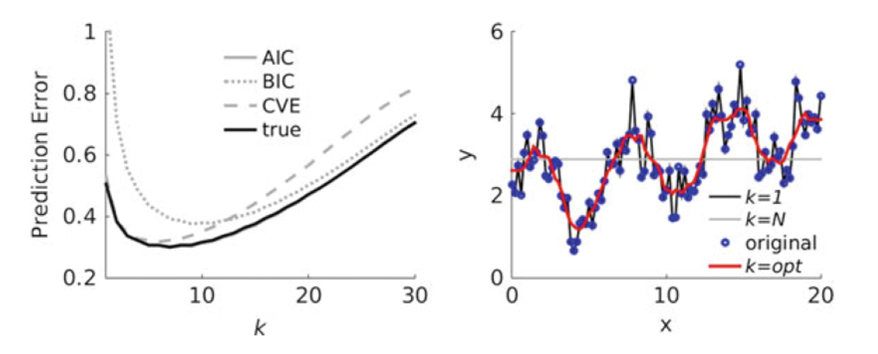
\includegraphics[width=0.7\textwidth]{figures/knn_reg.png}
    \caption{Information Criteria and Cross Validation estimates of the prediction error for KNN Regression.
    The larger $K$, the lower the number of effective parameters (lower model complexity). BIC is more conservative,
    choosing a less complex model (less risky regarding generalizability).}
    \label{fig:inf_knn_reg}
\end{figure}

\subsection{Breakpoint of Bias-Variance Tradeoff - double descent}
Usually, one would say \enquote{a model with zero training error is overfit to the training data and
will typically generalize poorly}. In double descent for (implicitly regularized models) a 
second descent in test error over complexity is observed in the overparameterized (data undersampled) regime
(depending on the dataset-model pair, more descents are possible).

\greenbox{\enquote{By considering larger function classes, which contain more 
candidate predictors compatible with the data, we are able to find interpolating 
functions that have smaller norm and are thus “simpler”. Thus increasing function 
class capacity improves performance of classifiers.} \citep{Belkin19}}

Double descent is illustrated in figure \ref{fig:double_descent}.

\begin{figure}[!htb]
    \centering
    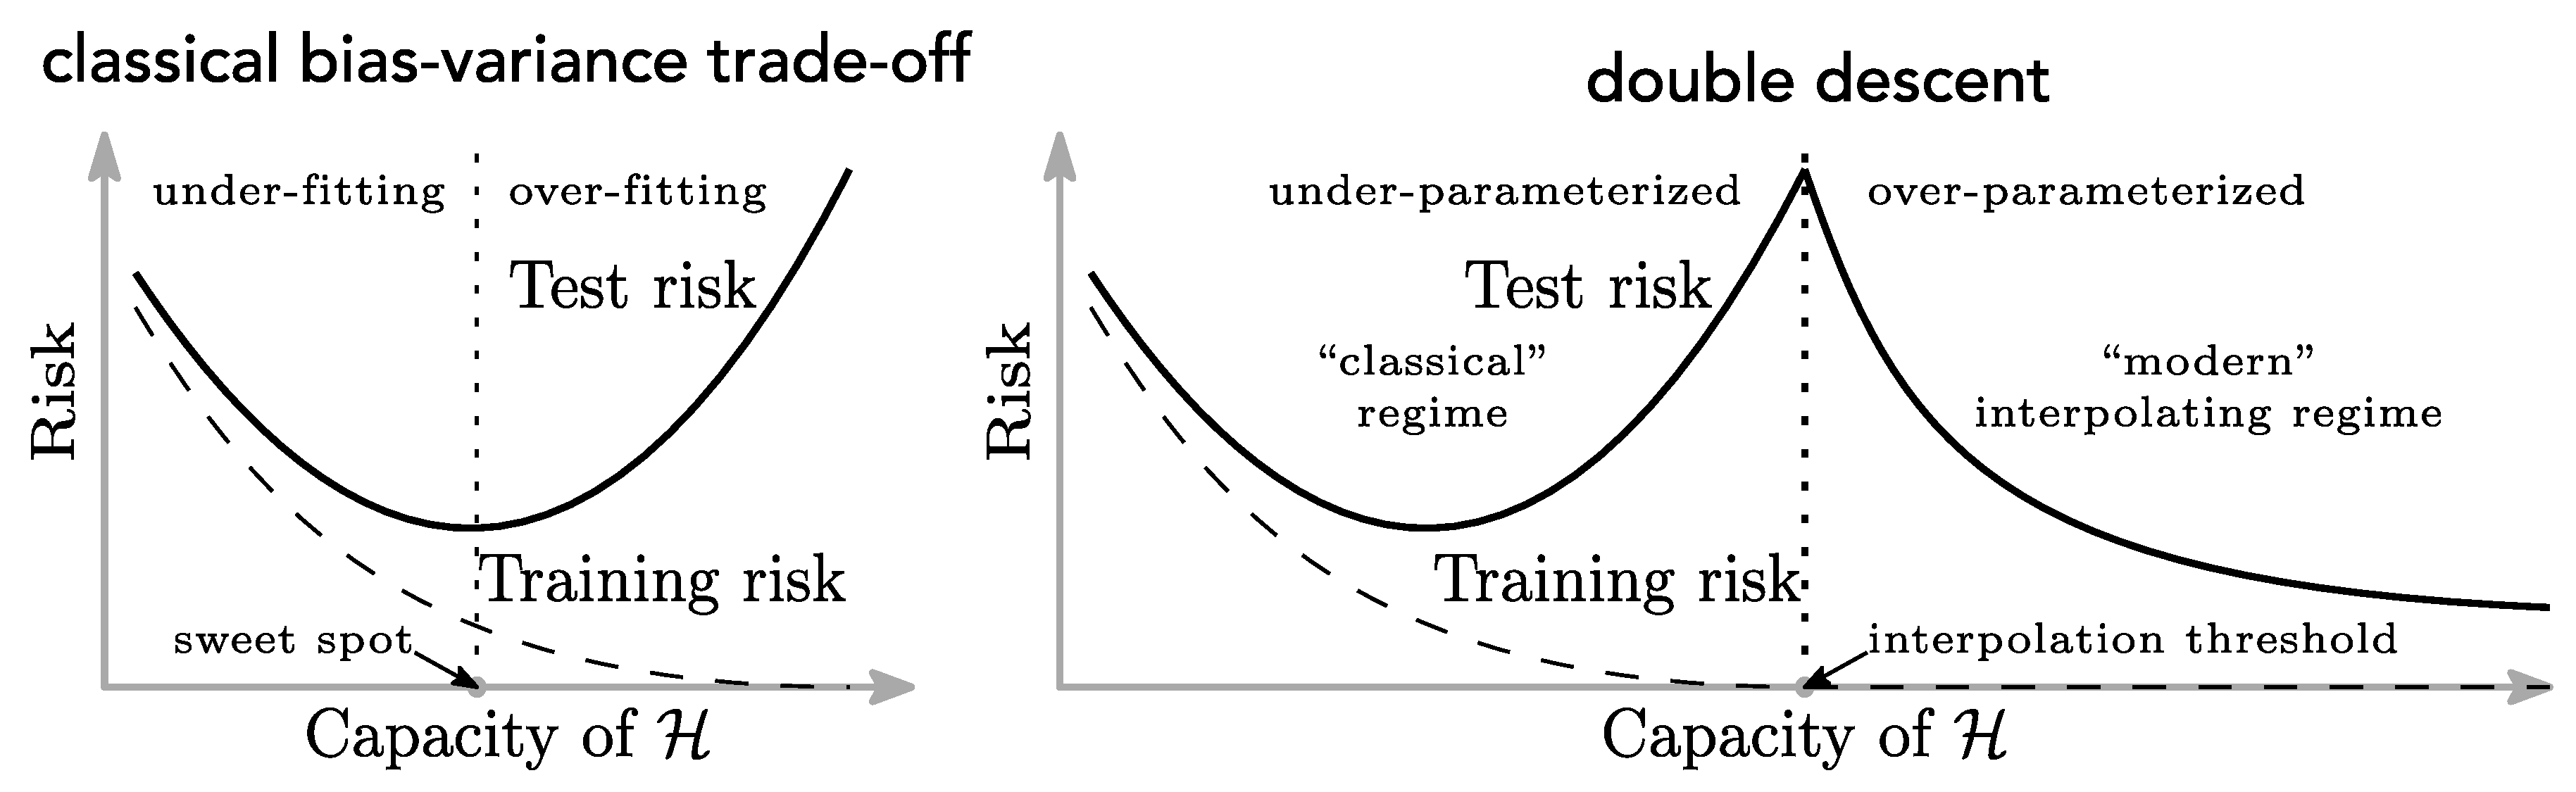
\includegraphics[width=0.95\textwidth]{figures/bvt.pdf}
    \caption{Double Descent in Test Error over Model Complexity}
    \label{fig:double_descent}
\end{figure}

\note{Double descent is not limited to complex neural networks but also
observed in ordinary overparameterized linear regression, see figure 
\ref{fig:double_descent_pol}.}

\begin{figure}[!htb]
    \centering
    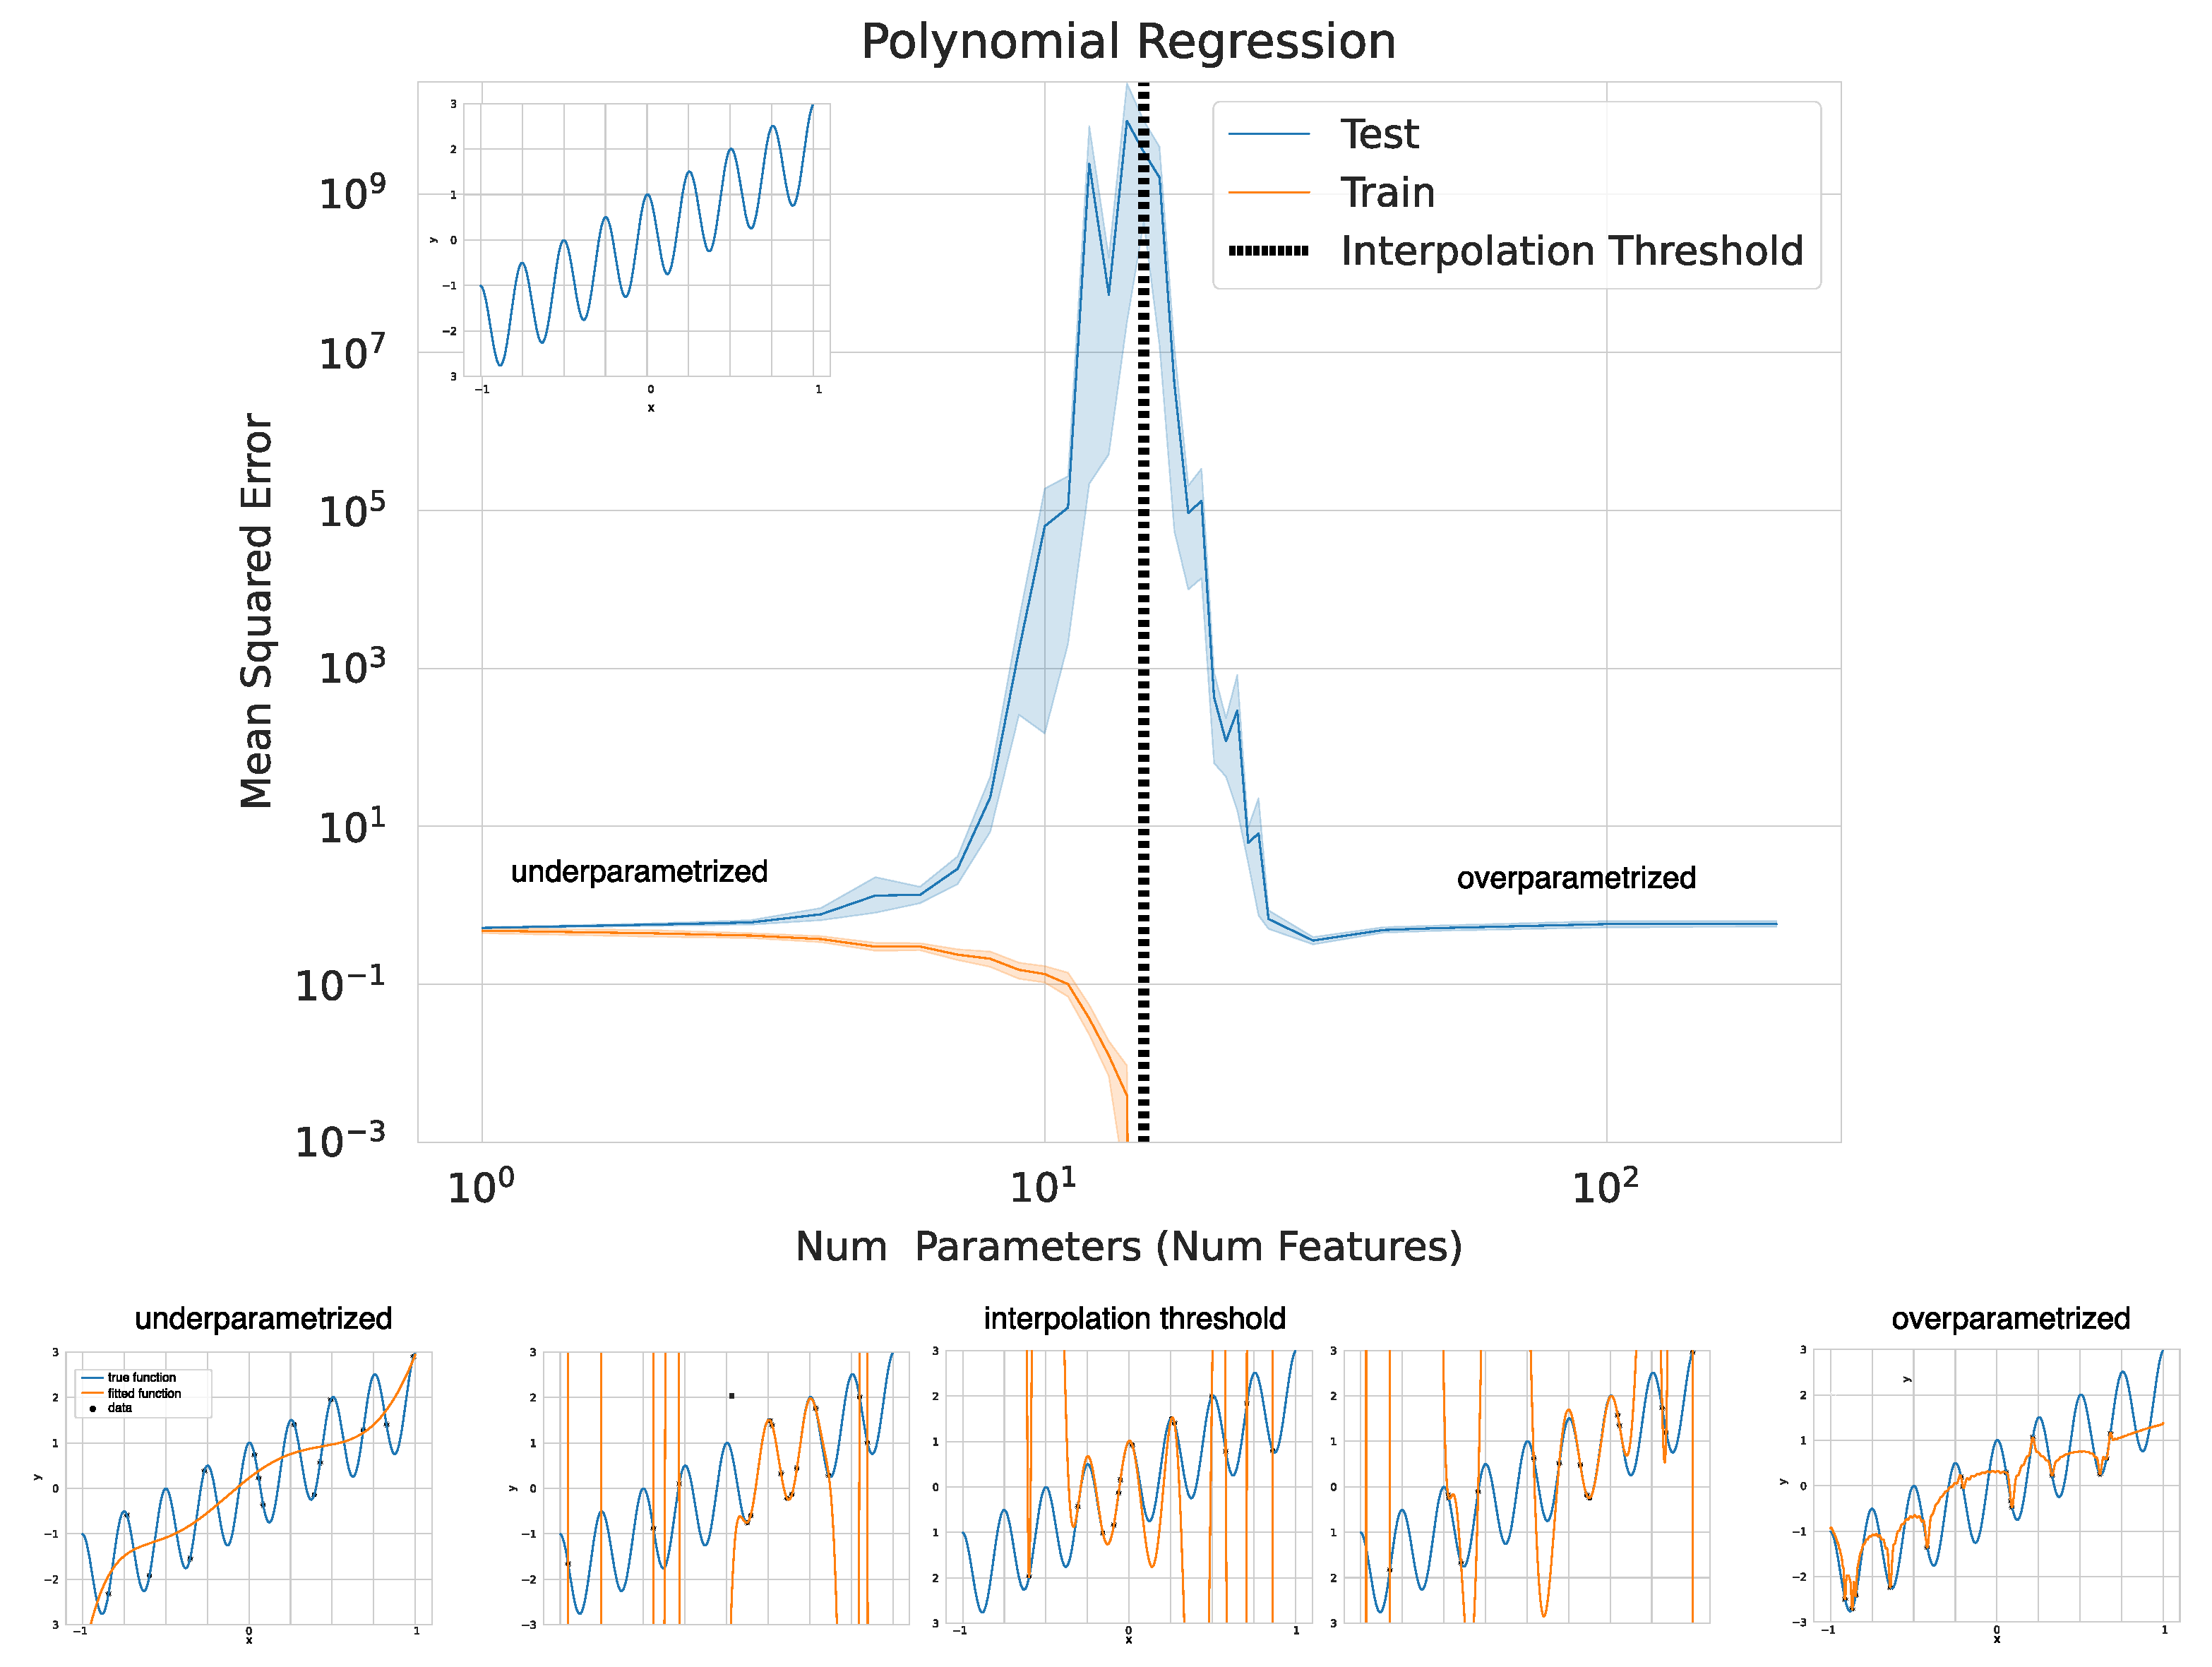
\includegraphics[width=0.95\textwidth]{figures/ddpr.pdf}
    \caption{In the overparameterized regime, the model can exactly fit the training data (small bias)
    but the model is also regularized towards a small-norm solution, making variance small.}
    \label{fig:double_descent_pol}
\end{figure}

\subsection{Curse of Dimensionality in Modeling\skipthis}
Curse of dimensionality is a term used to describe many phenomena.

\subsubsection{Curse of Dimensionality in Modeling / Sampling}
\begin{itemize}
    \item \textcolor{blue1}{Number of data points perspective}: Consider we find that to correctly model something in one dimension we need $N_1$ data points. Then in d dimensions we would need $N_1^d$ data points which quickly becomes infeasible with today's high-dimensional training data sets.
    \item \textcolor{blue1}{Resolvable scale perspective}: Consider we have a fixed number of data points $N$ sampling some distribution. Consider 
    our scale is the volume in which we expect to find one data point. For a box with length $L$, in one dimension, this scale is
    \begin{equation}
        \Delta x_{\text{1D}} = \frac{L}{N}, \quad \Delta x_{\text{2D}}^2 = \frac{L^2}{N} \quad \rightarrow \quad x_{\text{2D}} = \frac{L}{\sqrt{N}}
    \end{equation}
    so generally, in $d$ dimensions
    \begin{equation}
        x_{\text{dD}} = \frac{L}{N^{1/d}}
    \end{equation}
    So the higher the dimension, the worse our resolution for fixed $N$. This is illustrated in figure \ref{fig:curse_dens}.
\end{itemize}

\begin{figure}[!htb]
    \centering
    \includesvg[width=0.7\textwidth]{figures/curse_dens.svg}
    \caption{Curse of dimensionality in data density}
    \label{fig:curse_dens}
\end{figure}

\yellowbox{So we need more data to model things in higher dimensions. 
So classically, as number of features or dimensions grows, the amount 
of data we need to generalize accurately grows exponentially}

\subsubsection{Example for Curse of Dimensionality in number of possible models\skipthis}
Consider we are given
\begin{equation}
    \mat{X}=\left(\begin{array}{lll}
    0 & 0 & 0 \\
    0 & 0 & 1 \\
    0 & 1 & 0 \\
    0 & 1 & 1 \\
    1 & 0 & 0
    \end{array}\right), \quad \vec{Y}=\left(\begin{array}{l}
    0 \\
    1 \\
    1 \\
    0 \\
    1
    \end{array}\right)
\end{equation}
so data from a boolean function $f:\{0,1\}^3 \rightarrow \{0,1\}$.
There are $2^3$ possible inputs of such a function where a function
can give $2$ outputs so there are $2^{2^3} = 256$ possible boolean functions
of three variables. By fixing $5$ of the possible $8$ inputs, there are
still $2^3 = 8$ possible functions - which \textcolor{red1}{gets worse 
with more dimensions}.

\bluebox{For a model with more parameters than data points, we need regularization
to find the \textit{best no-bias model}.}

\subsection{Overview on dealing with complexity / model variance}

\problem{If not done right, more complex models with more parameters will tend to overfit, vary a lot
depending on the training set and generalize poorly.}

The higher the number of input features, the more complex the model will generally be, with 
the number of data points to retain the same sampling density growing exponentially with the number of features
(easy to see for e.g. a linear model). Now consider the model also has features in (higher dimensional)
\textit{latent spaces} - training will be even more difficult.

\greenbox{To make a model more robust (vary less) our principal approaches are
\begin{itemize}
    \item to train a simpler model
    on simpler data (less / more meaningful features) in the first place
    \item to penalize on model parameters / model output in some way, to reduce the sensitivity to noise / find the meaningful patterns / find a model with smoother simpler output
\end{itemize}}

\begin{itemize}
    \item \textcolor{blue1}{Feature selection}: Only use features (components of the measurements) relevant to the outcome, e.g. simply remove features with the least variance
    \item \textcolor{blue1}{Dimensionality reduction}: Project the data into lower dimensions which still capture 
    the relevant information (e.g. in semi-supervised learning train a dimensionality reduction on all data
    and in the lower dimensional space train a classifier on the labeled data)
    \item \textcolor{blue1}{Regularization}: Penalize model complexity / drive unnecessary parameters to zero
    \begin{itemize}
        \item Explicit regularization: add a term to the optimization problem, e.g. regularize on the norm of the model parameters or in physics informed regularization penalize how the model violates a differential equation
        \item Implicit regularization: other forms, e.g. early stopping in training a neural network (stop before model memorizes training data); dropout \footnote{Randomly ignore neurons during training (for a more robust distributed representation (?)).}; using stochastic gradient descent, ...
    \end{itemize}
\end{itemize}

\subsection{Feature selection - best subset selection}
Consider a data set $\mathcal{D} = \{(\vec{x}_i, y_i)\}_{i=1}^N$ with $\vec{x}_i \in \mathbb{R}^p$.

\begin{enumerate}
    \item Start with an empty set $S = \emptyset$
    \item Add a feature $\{ x_{ij} \}_{i=1}^N$ to $S$ which reduces the prediction error of the model the most
    \item Continue adding features until the prediction error rises again (overfitting)
    \item Backward elimination: As feature combinations added later might have made previous ones obsolete,
          one prunes $S \leftarrow S \setminus \{ x_{ij} \}_{i=1}^N$ as long as we can reduce the prediction error by doing so
\end{enumerate}

\subsection{Regularization I | General idea and pre-step}
\bluebox{\textbf{Aim:} Penalize model complexity to improve generalization.}
We penalize model complexity by modifying the loss to
\begin{equation}
    L_{\text{reg}} = L + \lambda \cdot \text{penalty}, \quad \text{regularization parameter } \lambda 
\end{equation}
where the penalty term is usually a $L_1$ or $L_2$ norm of the model parameters.
\subsubsection{Pre-step to regularization - centering, standardizing}
Consider the linear model
\begin{equation}
    y_i = \beta_0 + \sum_{j=1}^p \beta_j x_{ij} + \epsilon_i, \quad \mat{X} \in \mathbb{R}^{N \times p}, \vec{Y} \in \mathbb{R}^N
\end{equation}
Now consider we would like to regularize the model and driving down parameters of irrelevant features to zero.
\problem{\begin{itemize}
    \item the penalty term is not scale-invariant: consider two equally important features, one with a large numerical scale one with a small scale,
    in usual linear regression, the large-scale feature will have a smaller parameter but as of model linearity, the same effect on the prediction. But 
    consider we would drive small parameters to zero - then large scale features would be penalized more. So we scale and center the features in the feature matrix $\mat{X}$.
    \item we do not want to penalize the intercept term $\beta_0 = \bar{y} - \sum_{j=1}^p \bar{x}_j \beta_j$, so the response $\vec{Y}$ and features $\mat{X}$ should be centered
\end{itemize}}
\subsubsubsection{Centering and standardizing (z-scoring)}
\begin{equation}
    \begin{gathered}
        \tilde{\vec{x}}_i = \frac{\vec{x}_i - \bar{\vec{x}}}{\vec{s}_x}, \quad \bar{\vec{x}} = \frac{1}{N} \sum_{i=1}^N \vec{x}_i \\
        \tilde{y}_i = \frac{y_i - \bar{y}}{s_y}, \quad \bar{y} = \frac{1}{N} \sum_{i=1}^N y_i
    \end{gathered}
\end{equation}
where $\vec{s}_x$ collects the estimated standard deviations of the features (element-wise division).

\subsection{Bayesian perspective on Regularization}
\greenbox{Bayesian approaches guard from overfitting with the prior acting as a bias,
\textbf{the MAP in the Bayesian perspective is equivalent to a penalized maximum
likelihood, penalized with the logarithm of the prior}.}

\begin{equation}
    \begin{aligned}
        \vec{\hat{\beta}}_{\text{MLE,reg}} &= \argmin_{\vec{\beta}} \left(- \log \mathcal{L}(\vec{\beta}|\mat{X}) + \lambda P(\vec{\beta}) \right) \\
        \vec{\hat{\beta}}_{\text{MAP}} &= \argmin_{\vec{\beta}} \left( - \log{\left( \mathcal{L}(\vec{\beta}|\mat{X}) g(\vec{\beta}) \right)} \right) \\
        &= \argmin_{\vec{\beta}} \left( - \log{\left( \mathcal{L}(\vec{\beta}|\mat{X}) \right)} - \log{g(\vec{\beta})} \right) \\
    \end{aligned}
\end{equation}

where for $\vec{\hat{\beta}}_{\text{MAP}}$ the evidence $h(\mat{X})$ is constant and can be dropped.

Note, however, that in the Bayesian setting, the MAP plays no special role,
and if a point estimate is necessary, the posterior mean is usually preferred.

\subsection{Regularization II | Regularized regression}
\problem{Note that
\begin{itemize}
    \item for $p>N$, standard underparameterized linear regression breaks down, as $\mat{X}^T \mat{X}$ is not invertible
    \item for collinear features, there is also no unique solution to the parameters, consider e.g. bad training data
    \begin{equation}
        \vec{x}_i=\left(\begin{array}{c}
        1 \\
        x \\
        -x
        \end{array}\right) \rightarrow y=\beta_0+\beta_1 x-\beta_2 x=\beta_0+\left(\beta_1-\beta_2\right) x
    \end{equation}
    then there is a unique solution to $\beta_0, \beta_1 - \beta_2$ but not to $\beta_1, \beta_2$ separately.
    When the collinearity is not perfect, we might be able to invert $\mat{X}^T \mat{X}$ - but it is likely unstable, e.g.
    $\beta_1, \beta_2$ might be driven to very large values of opposite sign.
\end{itemize}
}

\idea{By regularization constrain the magnitude of the coefficients, bias towards smaller coefficients, so limiting
the problem of collinearity.}

\begin{equation}
    \begin{gathered}
        \vec{\hat{\beta}}_\text{regu} = \argmin_{\vec{\beta}} L = \argmin_{\vec{\beta}} \left( \operatorname{SSQ}(\vec{\beta}) + \lambda P(\vec{\beta}) \right) \\
        \operatorname{SSQ}(\vec{\beta}) = || \vec{Y} - \mat{X} \vec{\beta} ||^2, \quad \text{some penalty } P(\vec{\beta}) \\
        \text{regularization strength (hyperparameter)} \lambda
    \end{gathered}
\end{equation}

Different regularizations use different penalties.

\subsubsection{Ridge Regression}
We penalize on the squared norm of $\vec{\beta}$
\begin{equation}
    P(\vec{\beta}) = || \vec{\beta} ||_2^2 = \sum_{j=1}^p \beta_j^2
\end{equation}
So $\vec{\hat{\beta}}_\text{ridge}$ follows from
\begin{equation}
    \frac{\partial(\operatorname{SSQ}+\lambda P)}{\partial \vec{\beta}}=0 \rightarrow \vec{\hat{\beta}}_{\text {ridge }}=\left(\mat{X}^T \mat{X}+\lambda \mat{1}\right)^{-1} \mat{X}^T \vec{Y}=" \frac{\mat{X}^T \vec{Y}}{\mat{X}^T \mat{X}+\lambda \mat{1}} "
\end{equation}
\greenbox{\textbf{Intuition:} The regularization inflates the scatter matrix $\mat{X}^T \mat{X}$ (along all dimensions) by $\lambda$,
keeping the matrix invertible.}

\subsubsubsection{Influence of $\lambda$ and Bias-Variance Tradeoff}
With stronger regularization strenght $\lambda$, the parameters are driven towards zero, as 
illustrated in figure \ref{fig:ridge_reg_lambda}. The smaller the coefficients, the less sensitive
will the model output be to changes in the input, so the variance is reduced but the bias is increased.

For $\lambda \rightarrow 0$ we have
ordinary least squares linear regression. A sweet spot between bias and variance,
can be found by cross-validation.

This is illustrated in figure \ref{fig:ridge_reg_lambda}.

\begin{figure}[!htb]
    \centering
    \includesvg[width=0.95\textwidth]{figures/ridgel.svg}
    \caption{Ridge Regression - influence of $\lambda$ on the coefficients}
    \label{fig:ridge_reg_lambda}
\end{figure}

\subsubsubsection{Bayesian MAP perspective on Ridge regression}
Ridge regression is equivalent to the MAP estimate under the Gaussian error assumption using the prior
\begin{equation}
    \vec{\beta}_\text{prior} \sim \mathcal{N}(\vec{0}, \frac{\sigma^2}{\lambda} \mat{I})
\end{equation}
The larger $\lambda$ the more confident we are
one the \textit{initial guess} $\vec{\beta} = \vec{0}$. The corresponding negative log-likelihood of the prior is
\begin{equation}
    -\log p(\vec{\beta}) = \frac{1}{2} \vec{\beta}^T \frac{\lambda}{\sigma^2} \mat{I} \vec{\beta} = \frac{\lambda}{2 \sigma^2} || \vec{\beta} ||_2^2
\end{equation}
(where the $\frac{1}{\sigma^2}$ was used so it can me multiplied out from the minimization
together with the $\frac{1}{\sigma^2}$ in the term negative log-likelihood term).

\subsubsubsection{Discussion of the ridge regression}
\begin{itemize}
    \item bias is introduced
    \item \textcolor{green1}{stabilization:} coefficients for correlated features are pushed towards each other rather than
    one being wildly positive and the other wildly negative
    \item \textcolor{green1}{non important variables are pushed closer to zero}
    \item \textcolor{red1}{all variables are retained - no feature selection}
\end{itemize}

\subsubsection{On choosing the penalty}
In ridge regression, we used the $L_2$ norm in $P(\vec{\beta}) = || \vec{\beta} ||_2^2$.
More generally, we can use the $L_q$ norm
\begin{equation}
    P(\vec{\beta}) = || \vec{\beta} ||_q^q = \sum_{j=1}^p |\beta_j|^q
\end{equation}

Different norms are illustrated in figure \ref{fig:penalty_norms}.

\begin{figure}[!htb]
    \centering
    \includesvg[width=0.95\textwidth]{figures/penalty_norms.svg}
    \caption{Isocontours of $||\vec{\beta}||_q = 1$}
    \label{fig:penalty_norms}
\end{figure}

\subsubsection{Using the $L_0$ \textit{norm} (under $0^0 = 0$)}
The $L_0$ norm is the number of non-zero elements in a vector, so the 
number of explenantory variables used in the model - its not really a norm. Depending on 
the regularization strength, the $L_0$ norm drives us to using
less and less variables, as illustrated in figure \ref{fig:l0_norm_reg}.

\begin{figure}[!htb]
    \centering
    \includesvg[width=0.95\textwidth]{figures/l0_reg.svg}
    \caption{As $\lambda$ increases, we are first driven to the green, then to the blue estimate $\vec{\hat{\beta}}$ (drawn
    are the sum of squared residual contours).}
    \label{fig:l0_norm_reg}
\end{figure}

\problem{The $L_0$ norm is not convex (also not really a norm\footnote{Because it is not homogeneous, scaling $\vec{x}$ does not scale the norm.}) (and also not differentiable), so the optimization problem is not, so its
hard to optimize.}

\subsubsection{Lasso Regression}
\greenbox{A convex norm still selecting features is the $L_1$ norm, the sum of the absolute coefficient values.}
\subsubsubsection{Penalty in the Lasso - $L_1$ norm}
\begin{equation}
    P(\vec{\beta}) = || \vec{\beta} ||_1 = \sum_{j=1}^p |\beta_j| = \operatorname{sign}(\vec{\beta})^T \vec{\beta}, \quad [\operatorname{sign}(\underline{\beta})]_i= \begin{cases}-1, & \beta_i<0 \\ 0, & \beta_i=0 \\ 1, & \beta_i>0\end{cases}
\end{equation}

\subsubsubsection{Why does Lasso drive coefficients to exactly zero? | Soft-thresholding of the coefficients in Lasso regression}
\yellowbox{Lasso regression sets coefficients to exactly zero. This can
be written as a soft-thresholding one the ordinary least squares solution,
setting sufficiently small coefficients to zero.}

For $P(\vec{\beta}) = || \vec{\beta} ||_1$, the loss becomes

\begin{equation}
    L(\vec{\beta}) = \operatorname{SSQ}(\vec{\beta}) + \lambda || \vec{\beta} ||_1 = || \vec{Y} - \mat{X} \vec{\beta} ||^2 + \lambda || \vec{\beta} ||_1
\end{equation}

\note{$|| \vec{\beta} ||_1$ is not differentiable at zero, so in the following assume $\beta_j \neq 0$. By consistency argumentation
we can then say, when we should have $\beta_j = 0$.}

\begin{equation}
    \partial_\vec{\beta} L = -2 \mat{X}^T \vec{Y} + 2 \mat{X}^T \mat{X} \vec{\beta} + \lambda \mat{D} \vec{1} \underset{!}{=} 0, \quad D_{jj} = \begin{cases} 1, & \beta_j > 0 \\ -1, & \beta_j < 0 \end{cases}
\end{equation}

which also places the constraint
\begin{equation}
    D_{jj} = \operatorname{sign}(\beta_j)
\end{equation}

\paragraph{Derivation of the thresholding for scalar $x_i \in \mathbb{R}$, so $\beta \in \mathbb{R}$ ($\beta_0 = 0$ as we centered the data)} In 1D
we have
\begin{equation}
    \begin{aligned}
    & \frac{\partial \mathcal{L}}{\partial \underline{\beta}}=-2 \sum_{i=1}^N x_i y_i+2 \beta \sum_{i=1}^N x_i^2+\lambda d=0, \quad d=\left\{\begin{array}{cc}
    -1, & \beta<0 \\
    1, & \beta>0
    \end{array}\right. \\
    & \rightarrow \hat{\beta}_{\text {lasso }}=\frac{\sum_{i=1}^N x_i y_i}{\sum_{i=1}^N x_i^2}-\frac{\lambda d}{2 \sum_{i=1}^N x_i^2}=\hat{\beta}_{M L E}-\frac{\lambda d}{2 \sum_{i=1}^N x_i^2} \\
    &
    \end{aligned}
\end{equation}

Consistency of $\beta_{\text{lasso}}$ with the sign of $d$ requires
\begin{equation}
    d=1 \rightarrow \hat{\beta}_{M L E}>\frac{\lambda}{2 \sum_{i=1}^N x_i^2}, \quad d=-1 \rightarrow \hat{\beta}_{M L E}<-\frac{\lambda}{2 \sum_{i=1}^N x_i^2}
\end{equation}

\bluebox{So if $\hat{\beta}_\text{lasso}$ is to be non-zero, $\hat{\beta}_\text{MLE}$ must be larger (in magnitude) than a certain value. 
So otherwise, $\hat{\beta}_\text{lasso}$ is set to zero.}

\note{The equation derived above for $d=0$ so $\hat{\beta}_\text{lasso} = 0$ says $\hat{\beta}_\text{MLE} = 0$, a contradiction so 
it seems. But note that the equation is derived for $\beta \neq 0$, as of differentiability, so inserting $d = 0$ is not even valid.}

This is illustrated in figure \ref{fig:lasso_reg}.

\begin{figure}[!htb]
    \centering
    \includesvg[width=0.95\textwidth]{figures/lasso_soft2.svg}
    \caption{Soft thresholding in Lasso regression}
    \label{fig:lasso_reg}
\end{figure}

Loss contours of lasso regressio and ridge regression are illustrated in figure \ref{fig:ridge_lasso_contours}.

\begin{figure}[!htb]
    \centering
    \includesvg[width=0.8\textwidth]{figures/ridge_lasso_contours.svg}
    \caption{Loss contours of lasso and ridge regression}
    \label{fig:ridge_lasso_contours}
\end{figure}

\subsubsubsection{Influence of $\lambda$ on the coefficients in Lasso regression}
The feature selection performed by Lasso is illustrated in figure \ref{fig:lasso_lambda}.

\begin{figure}[!htb]
    \centering
    \includesvg[width=0.95\textwidth]{figures/lassolambda.svg}
    \caption{Influence of $\lambda$ on the coefficients in Lasso regression}
    \label{fig:lasso_lambda}
\end{figure}

For strongly correlated features, one is often pushed fully to zero.

\subsubsection{Why does Lasso regression lead to feature selection (\textit{induces sparsity}) and Ridge regression does not?}
We have already gaines some intuition, why by consistency in Lasso regression, coefficients are driven to zero.
Another angle comes from the constraint perspective.

\subsubsubsection{Constraint perspective and regularized regression}
The \textbf{Ridge minimization}
\begin{equation}
    \vec{\hat{\beta}}_{\text{ridge},\lambda} = \argmin_{\vec{\beta}} \left( \operatorname{SSQ}( \vec{\beta}) + \lambda || \vec{\beta} ||_2^2 \right)
\end{equation}
can be written as as the constraint optimization problem
\begin{equation}
    \vec{\hat{\beta}}_{\text{ridge},\gamma} = \argmin_{\vec{\beta}} \operatorname{SSQ}(\vec{\beta}) \quad \text{s.t.} \quad || \vec{\beta} ||_2^2 \leq \gamma
\end{equation}
where
\begin{equation}
    \forall \lambda > 0 \quad \exists \gamma: \vec{\hat{\beta}}_{\text{ridge},\lambda} = \vec{\hat{\beta}}_{\text{ridge},\gamma}
\end{equation}

The \textbf{Lasso minimization}
\begin{equation}
    \vec{\hat{\beta}}_{\text{lasso},\lambda} = \argmin_{\vec{\beta}} \left( \operatorname{SSQ}( \vec{\beta}) + \lambda || \vec{\beta} ||_1 \right)
\end{equation}
can analogously be written as as the constraint optimization problem
\begin{equation}
    \vec{\hat{\beta}}_{\text{lasso},\gamma} = \argmin_{\vec{\beta}} \operatorname{SSQ}(\vec{\beta}) \quad \text{s.t.} \quad || \vec{\beta} ||_1 \leq \gamma
\end{equation}
where
\begin{equation}
    \forall \lambda > 0 \quad \exists \gamma: \vec{\hat{\beta}}_{\text{lasso},\lambda} = \vec{\hat{\beta}}_{\text{lasso},\gamma}
\end{equation}

\bluebox{In the constraint perspective, $\vec{\hat{\beta}}_{\gamma}$ is the value of $\vec{\beta}$ which minimizes the sum of squared residuals,
and lies withing the contour $|| \vec{\beta} ||_q^q = \gamma$, so $|| \vec{\beta} ||_2^2 \leq \gamma$ for Ridge and $|| \vec{\beta} ||_1 \geq \gamma$ for Lasso.}

\subsubsubsection{Intuition for the difference in feature selection}
The constraint solution found is the point of intersection of the first isocontour of the sum of squared residuals and
the constraining contour. For the Lasso regression, the constraining contour is a diamond, so the intersection
is more likely to be on the axis, so at least one coefficient is set to zero. This is illustrated in figure \ref{fig:ridge_lasso_constraint}.

\begin{figure}[!htb]
    \centering
    \includesvg[width=0.95\textwidth]{figures/ridge_lasso_constraint.svg}
    \caption{Sum of squares contours and constraining contours for Ridge and Lasso regression. If the OLS estimate falls within one of
    the green-shaded areas, one parameter is set to zero in Lasso Regression. This is not the case for Ridge regression.}
    \label{fig:ridge_lasso_constraint}
\end{figure}

\subsection{Preview: Fighting overfitting and improving performance in Neural Networks: Dropout}
By randomly leaving out connections / neurons in a neural network a more distributed representation
and robust solutions can be obtained.

\pagebreak